\documentclass[border=2pt]{standalone}
\usepackage{tikz}
\usetikzlibrary{positioning}
\begin{document}
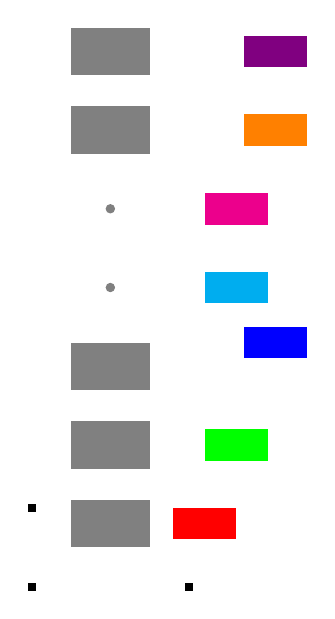
\begin{tikzpicture}[
  base/.style={fill=gray,minimum width=10mm,minimum height=6mm,inner sep=0pt,outer sep=0pt},
  probe/.style={minimum width=8mm,minimum height=4mm,inner sep=0pt,outer sep=0pt}]
  % Calibration marks: centers at (0,0), (20,0), (0,10) in physical mm.
  \fill (-.5mm,-.5mm) rectangle (.5mm,.5mm);
  \fill (19.5mm,-.5mm) rectangle (20.5mm,.5mm);
  \fill (-.5mm,9.5mm) rectangle (.5mm,10.5mm);
  \node[base] (a) at (10mm,8mm) {};
  \node[base] (b) at (10mm,18mm) {};
  \node[base] (c) at (10mm,28mm) {};
  \coordinate (pin) at (10mm,38mm);
  \fill[gray] (10mm,38mm) circle[radius=.6mm];
  \fill[gray] (10mm,48mm) circle[radius=.6mm];
  \node[base] (f) at (10mm,58mm) {};
  \node[base] (g) at (10mm,68mm) {};
  \node[probe,fill=red,on grid,right=12mm of a] {};
  \node[probe,fill=green,on grid,right=12mm of b.center] {};
  \node[probe,fill=blue,on grid,right=12mm of c.north east] {};
  \node[probe,fill=cyan,on grid,right=12mm of pin] {};
  \node[probe,fill=magenta,on grid,right=12mm of {10mm,48mm}] {};
  \node[probe,fill=orange,right=12mm of f] {};
  \node[probe,fill=violet,right=12mm of g,on grid] {};
\end{tikzpicture}
\end{document}
